
\documentclass[aps,prl,reprint]{revtex4-2}
\usepackage{gensymb}
\usepackage{graphicx}
\usepackage{amsmath}
\usepackage{hyperref}
\usepackage{dsfont}
\usepackage{relsize}
\usepackage{wrapfig}
\usepackage{graphicx}
\usepackage{hyperref}
\hypersetup{colorlinks=true, citecolor=blue, urlcolor=blue, linkcolor=blue}


\begin{document}

% Use the \preprint command to place your local institutional report
% number in the upper righthand corner of the title page in preprint mode.
% Multiple \preprint commands are allowed.
% Use the 'preprintnumbers' class option to override journal defaults
% to display numbers if necessary
%\preprint{}

%Title of paper
\title{Coupled Electric Oscillators}

% repeat the \author .. \affiliation  etc. as needed
% \email, \thanks, \homepage, \altaffiliation all apply to the current
% author. Explanatory text should go in the []'s, actual e-mail
% address or url should go in the {}'s for \email and \homepage.
% Please use the appropriate macro foreach each type of information

% \affiliation command applies to all authors since the last
% \affiliation command. The \affiliation command should follow the
% other information
% \affiliation can be followed by \email, \homepage, \thanks as well.
\author{Trevor Smith, Alex Storrer}
\email[]{smith.tr@northeastern.edu}
\homepage[]{https://github.com/trevorm4x/}
%\thanks{}
%\altaffiliation{}
\affiliation{Northeastern University}


\date{\today}

\begin{abstract}

	In this lab, the behavior of single, uncoupled, and coupled LRC circuits
	were evaluated with simple relationships between L, R, C, and voltage
	as well as complex differential equations. The latter were simplified
	based on the unique initial conditions of this experiment. This behavior
	was further linked to a mechanical analogue, an elastic pendulum system.
	For two inductors, nearly identical behavior of the single RLC circuit was
	observed.  The oscillating decay of the single LRC
	circuits  were  similar  for  the  two  inductors, where A-inductor
	and B-inductor were calculated to have decay  natural 
	frequencies  of  14587.05$\pm$ 0.03  rad/sec and 14578.44$\pm$ 0.03 rad/s, and
	decay constants of 649.9$\pm$ 0.1 s−1 and 651.3$\pm$ 0.1 s−1.  From these
	values the inductances were calculated to be 0.100±0.003 H for both of 
	the inductors. When the A and B circuits were coupled via a coupling
	capacitor, each circuit produced a signal with a beat frequency of 
	170 $\pm$ 1 Hz. By using equations modeling a coupled LRC circuit, the
	coupling capacitance was calculated to be 4.1 $\pm$ 0.1 nF, which is one
	standard deviation away from its measured value of 3.9 $\pm$ 0.1 nF.

\end{abstract}


\maketitle

% body of paper here - Use proper section commands
% References should be done using the \cite, \ref, and \label commands
\section{Introduction}
% The Introduction should contain 1 or 2 paragraphs.
% Briefly state the physics underlying the experiment
% (what is being tested and why). 
In many circuits, a voltage is continuously applied to several components in series 
and/or in parallel. Three essential components used in circuits are resistors, 
capacitors, and inductors. These components operate in distinct ways, which can be
seen by the way we use inductance, resistance, and capacitance to calculate voltage.

$$ V = L \cdot \frac{d^2q}{dt^2} $$
$$ V = R \cdot \frac{dq}{dt} $$
$$ V = \frac{1}{C} \cdot q $$

Where V is voltage, L is inductance, R is resistance, C is capacitance, and q is 
charge. In other words, capacitors do work proportional to amount of charge buildup, 
resistors do work proportional to the flow of charge or current, and inductors do 
work proporional to the inflection of charge, or the change in current. \\

\begin{figure}[h]
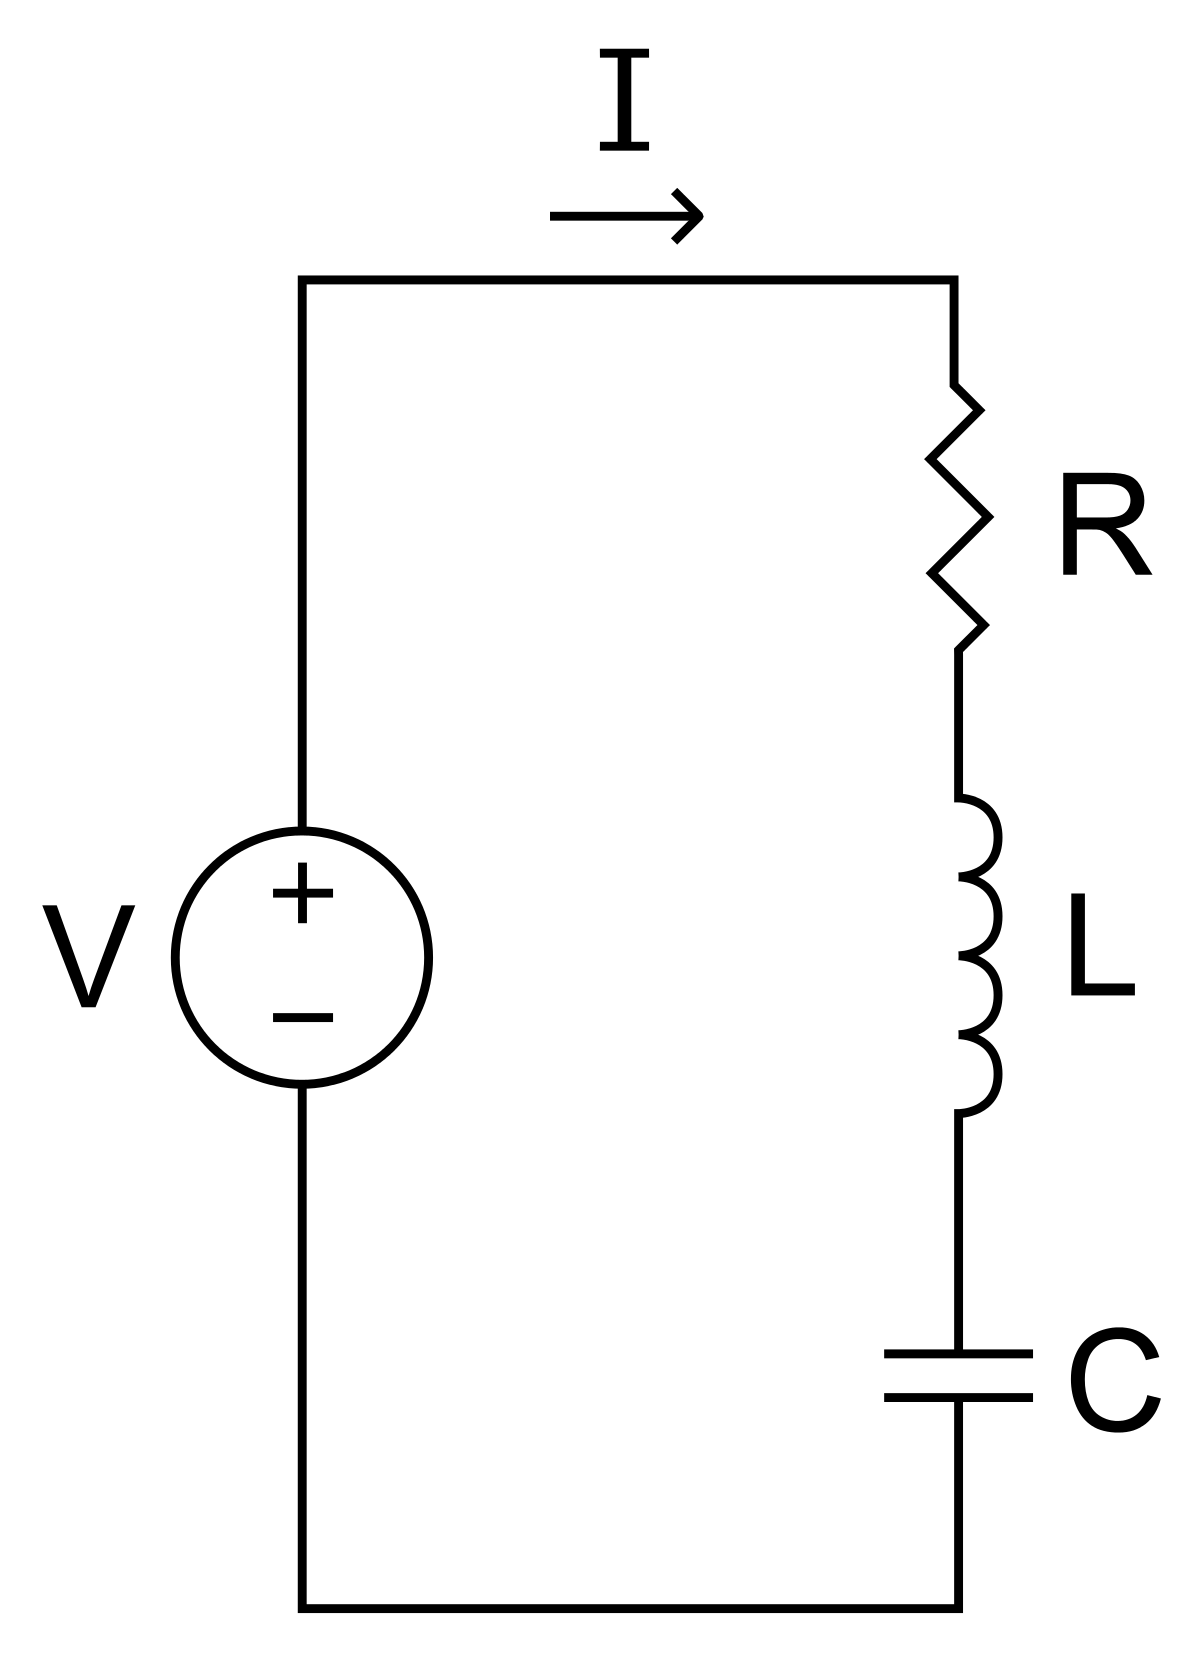
\includegraphics[width=0.4\textwidth]{../Images/l6_LRC.png}
\caption{\label{figA}}
\end{figure}

An LRC circuit, seen in \ref{figA}, combines these three components to produce an 
oscillating response
to any change in voltage, for example the turning on and off of an applied voltage.
These oscillations could be compared to the oscillation of a spring-mass system,
and indeed the differential equations describing both the voltage of an LRC circuit
and the height of an oscillating spring/mass system in gravity look identical. \\

This peculiar behavior can be multiplied when two such systems interact with each 
other, behaving as what's known as ``coupled oscillators". The beauty of differential
equations is that a mathematical model can be used to describe such motion, even
if the differential equation itself is unsolvable unless there are specific initial
parameters. In an unsolvable case, a computer program can simulate the system one step at a
time using Euler's method, or we can simply perform an experiment and let nature 
describe the motion. In this lab, we will be looking at a coupled electric oscillator
that is operating in a normal mode, which is to say a mode where the coupled oscillators
behave like a single harmonic oscillator, or a solvable case.




\section{Apparatus}
% List equipment components (manufacturer, model
% numbers and brief specifications). 

The apparatus consisted of the following.
\begin{itemize}
	\item Coupled electronic oscillator circuit box
	\item Fixed capacitor, variable capacitor
	\item Two large inductor coils, labelled 'A' and 'B'
	\item Oscilloscope, Tektronix TDS210 
	\item Digital Multimeter, Extech EX430A
	\item OpenChoice Desktop, Oscilloscope Software
	\item Jupyter, Python compiler
	\item LaTeX, document preparation software
\end{itemize}

\section{Measure Inductance}

\subsection{Procedure}
% Briefly describe the experimental procedures (in your own words, but don’t overdo it)
% Discuss calibrations, etc., if required
% Include necessary equations and put them on their own line (number them, e.g. “Eq. (3)”)
% Include plots showing relevant results (label each figure, e.g. “Fig. 3”, with caption).
% Describe what you found (describe what the plot illustrates)
In this phase of the lab we measure the basic parameters of our system, described
in \ref{setup}, including $L_A$, $L_B$, $R_L_A$, $R_L_B$, full decay natural 
frequency $\omega_0$, damping constant $\gamma$, time constant $\tau$, 
quality factor $Q$ and the standard capacitor. These values, save for the capacitance,
are calculated by analyzing the voltage oscillations of the circuit. Values for $R_L_A$
and $R_L_B$ are also measured with an ohmmeter, and the capacitance is measured
with a digital multimeter (DMM). \\

\begin{figure}[h]
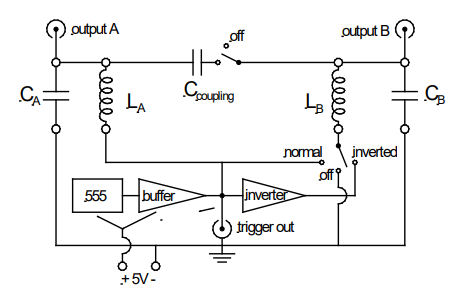
\includegraphics[width=0.4\textwidth]{../Images/l6_setup.png}
\caption{\label{setup} Test setup for the coupled electric oscillators.}
\end{figure}

The standard capacitor and one inductor was installed in the A-circuit. A +5 VDC source
was connected to the box, and the A-output was connected to channel 1 of an oscilloscope.
The trigger out was connected to the scope trigger, and the viewing window of the scope
was adjusted so that the decaying oscillation occurring when the square wave turns off
was visible. \\

The decaying waveform is then stored digitally and analyzed. By using eq. 
\ref{LRC Oscillation} to make curve fits, the basic parameters of the system
can be obtained. These fits were first performed on a single period of oscillation,
in order to get an estimate without the added complexity of the exponential. Then,
using the parameters for the sine wave as a starting point, the full equation describing
the oscillation was obtained.

\begin{equation} 
q(t) = q_{0}e^{-\gamma t/2}cos(\omega_0t)
\label{LRC Oscillation}
\end{equation}

Where q is charge as a function of time, $\gamma$ is the decay constant,
$\omega_0$ is the natural frequency, and t is time. This equation,
analogous to a mass-spring system being stretched and released,
describes the flow of charge between the capacitor and inductor in
the LRC circuit. When the `spring is released', or the 555 pulse
square wave switches off, the capacitor immediately discharges.
However, the inductor counters such a quick change in current,
and produces a current in the opposite direction, cancelling out a
portion of the flow of charge from the capacitor. This has the 
effect of recharging the capacitor again, which, when the flow
of current from the inductor is stopped, will again quickly
discharge. The length of wire between the two circuit components,
in this case, acts as a resistor and steadily gives off energy
in the form of heat as a proportion of the current at a given
moment. The end result is this beautiful equation 
describing a sine wave undergoing exponential decay. \\

This analysis was repeated with inductor `B', inserted into the same circuit
and replacing inductor `A'.

\subsection{Results}

First, the capacitance of the standard capacitor was measured. The DMM has an
uncertainty of 3\% associated with all measurements, and yielded a capacitance
measurement of 47 $\pm$ 1 $\mu$F. \\

A single period of the oscillation was recorded and analyzed for each inductor,
shown in \ref{single_period}. 

\begin{figure}[h]
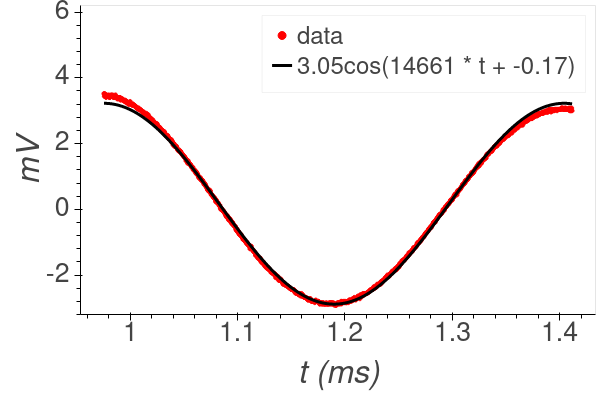
\includegraphics[width=0.4\textwidth]{../Images/l6_channel_A_one_period_fit.png}
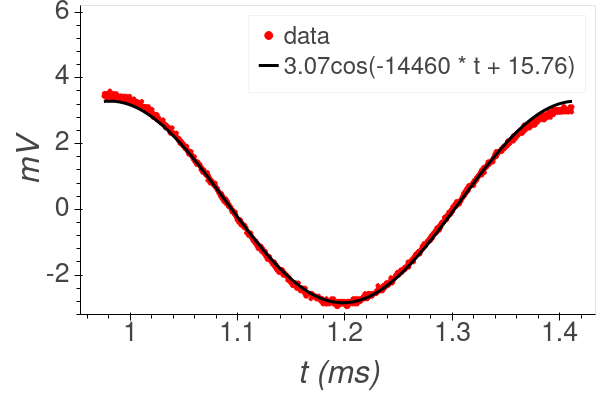
\includegraphics[width=0.4\textwidth]{../Images/l6_channel_B_one_period_fit.png}
\caption{\label{single_period} Single period of oscillation and fit for A (above) and B
(below). The differing fit parameters for phase and the sign of the frequency is not
relevant in this case. }
\end{figure}

\newpage
The calculated frequencies for A and B, respectively, are 14660 $\pm$ 30 Hz and
14460 $\pm$ 30 Hz, where the uncertainty is calculated from the covariance
matrix of the fit. Using \ref{LCalc} and the values above, $L_A$ and $L_B$ were
calculated to be 0.099 $\pm$ 0.003 H and 0.101 $\pm$ 0.003 H. It should be noted
that the uncertainty in the fit was well below one part in 100, meaning that
nearly all the uncertainty in the inductance measurements were due to the DMM.

\begin{equation} 
	L = \frac{1}{C\omega_0^2}
	\label{LCalc}
\end{equation}

These fit parameters were then used as starting parameters for the more complicated
curve fit needed when exponential decay is included, as shown in \ref{full}. 

\begin{figure}[h]
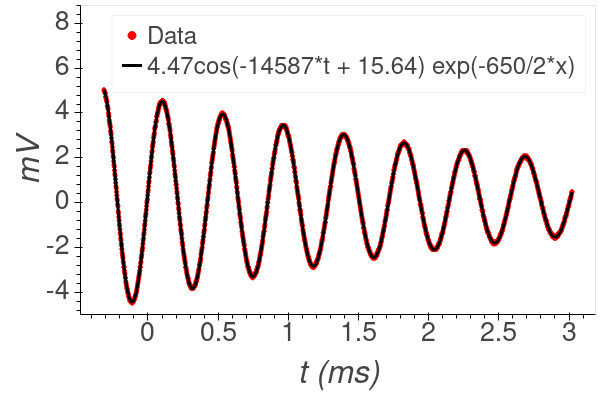
\includegraphics[width=0.4\textwidth]{../Images/l6_channel_A_full_fit.png}
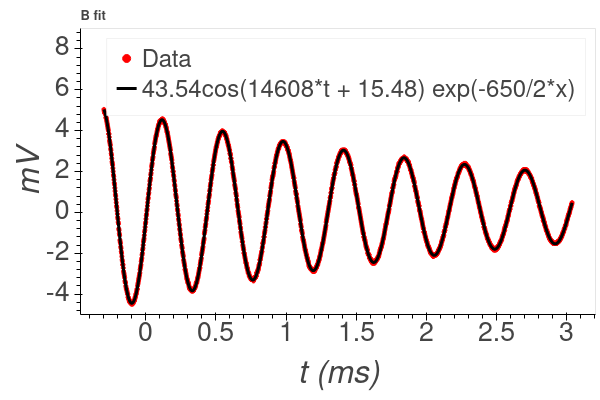
\includegraphics[width=0.4\textwidth]{../Images/l6_channel_B_full_fit.png}
\caption{\label{full} Several periods of oscillations, with fit corresponding
to eq. \ref{LRC Oscillation}. }
\end{figure}

While the frequencies for A and B when viewing a longer decay
were extremely precise, 14587.05 $\pm$ 0.03 and 14578.44 $\pm$ 0.03
respectively, the proportion of uncertainty in our calculated
L values were exactly the same, caused again by uncertainty in the
measured capacitance. These values did, however, agree better than
before, at $0.100\ \pm\ 0.003$ H for both inductors. \\

The damping coefficient $\gamma$ was calculated at 650 /s and 651 /s for
A and B respectively. This damping coefficient $\gamma$ is related to the
resistance R, which generates heat proportional to the flow of charge,
and inductance L which generates a flow of charge opposite to the
change in current, by eq. \ref{LRG}. We can then rearrange the equation
so that we can use our calculated inductance and frequency to calculate
resistance.

\begin{equation} 
	\gamma = \frac{R}{L} \rightarrow R = L\gamma 
	\label{LRG}
\end{equation}

The resistance for inductor `A' and `B' were both found to be 
$65\ \pm\ 2\ \Omega$. Again, calculations were precise enough
to be able to distinguish a difference in the damping coefficient
itself for the two inductors, but the error propagated from the 
DMM swamps that difference. This difference is small when considering
the discrepancy between these calculated values for resistance and
those measured directly with an ohmmeter. These measured resistances
for inductor `A' and `B' were 17.4 $\pm$ 0.2 $\Omega$ and
17.2 $\pm$ 0.2 $\Omega$ respectively, with the error again coming from
the DMM's 3\% precision. \\

This difference can be attributed to a difference in exactly what 
is being measured. In the case of the DMM, the inductors were isolated
from the circuit and measured separately, whereas the decay constant 
is caused by all resistance that exists in the circuit, including the
wire and all contacts. Therefore, it is not surprising that the
resistance related to the time constant is much higher. \\

In theory, this resistance does not have any effect on the frequency
of the circuit, as $\omega_0$ is clearly a function of only L and C. \\

Finally, two more important values were derived from values already
discussed, $\tau$, another to describe damping, called the time constant,
and $Q$, or the quality factor, which also describes the decay
in an oscillating system. The equations used for these values are given
by \ref{tau} and \ref{Q} respectively.
All constants in these equations have already been defined in this report.

\begin{equation} 
	\tau = \frac{2}{\gamma}
	\label{tau}
\end{equation}

\begin{equation} 
	Q = \frac{\omega_0}{\gamma}
	\label{Q}
\end{equation}

The quality factor for circuits containing each inductor `A' and `B' were
again found to be equal after considering uncertainty due to the DMM,
at 22.4 $\pm$ 0.7. This value corresponds to the amount of decay that
occurs over a single period. \\

The time constant for circuits containing each inductor `A' and `B' 
calculated with great precision, as they do not depend on any measurements
from the DMM. These values were 0.0030773 $\pm$ 0.0000006 s and 
0.0030709 $\pm$ 0.0000006 s respectively. These uncertainties are 
$6.0\ \cdot\ 10^{-7}$.

\newpage
\section{Uncoupled LRC Oscillators}

In the following sections, a system with two LRC circuits will be
analyzed, starting with two uncoupled LRC oscillators.
The B inductor and adjustable capacitor were then added to the 
B-circuit, and the B-circuit output was connected to channel
2 on the scope. By switching the coupling capacitor 
\textbf{\emph{off}}, these two LRC circuits were able to operate
independently, but excited by the same emf pulse.\\

The waveforms were viewed on the oscilloscope, and the B-capacitor
was adjusted until both waveforms had the same period. These
waveforms were stored and are shown in fig. \ref{same}.

\begin{figure}[h]
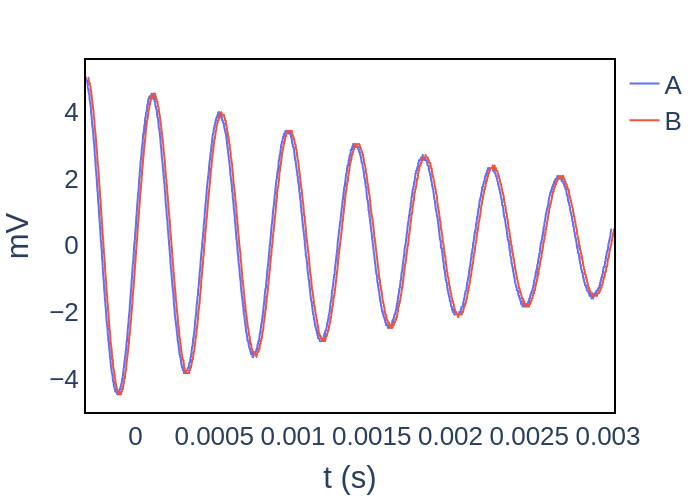
\includegraphics[width=0.4\textwidth]{../Images/l6_uncoupled_full_window.png}
\caption{\label{same} Two uncoupled LRC circuits powered by the same pulse 
generator. }
\end{figure}

The variable capacitor was then removed from the circuit and measured
with the DMM at 47 $\pm$ 1 nF. Considering that this value is exactly
the same as the standard capacitor, and that the two inductances
were the same within uncertainty, this makes sense. We would expect
that, if all other parameters describing the oscillation are
more or less equal, then in order to equalize the resulting waves
then this parameter would need to be equal as well.


\section{Coupled LRC Oscillator}

In the final phase of this experiment, two coupled LRC oscillators
are analyzed. The complexity of this system is drastically higher
than a single oscillator, and as such the circuit has been designed
in such a way to simplify the interaction of the two LRC circuits
in terms of their phase. In the ``normal" configuration, 
the amplitude of on oscillators are either the same or exactly
opposite, corresponding to a phase difference of 0 or 180 degrees.
In this configuration, the A-circuit begins at a maximum and
the B-circuit begins at zero, corresponding to a 90 degrees phase 
difference. This is achieved by switching ``on" the coupling in
our box, but switching ``off" the trigger connection to the 
B-circuit. \\

\subsection{Observing the ``Beat"}

\subsubsection{Procedure}

In this portion of the lab, we will observe the resulting output
of the coupled LRC circuits and attempt to explain its behavior.\\

The variable capacitor was replaced in the B-circuit, and 
the box was set to the above stated parameters.  As in the first 
section, the window of the scope was moved to observe only the
falling edge of the excitation and the ensuing behavior of the
two coupled circuits. The variable capacitor was tuned to reduce
the minima between the resulting waves closest to zero as possible.\\

\subsubsection{Results}

The resulting waves were saved and analyzed digitally, and can be seen
in \ref{waves}.

\begin{figure}[h]
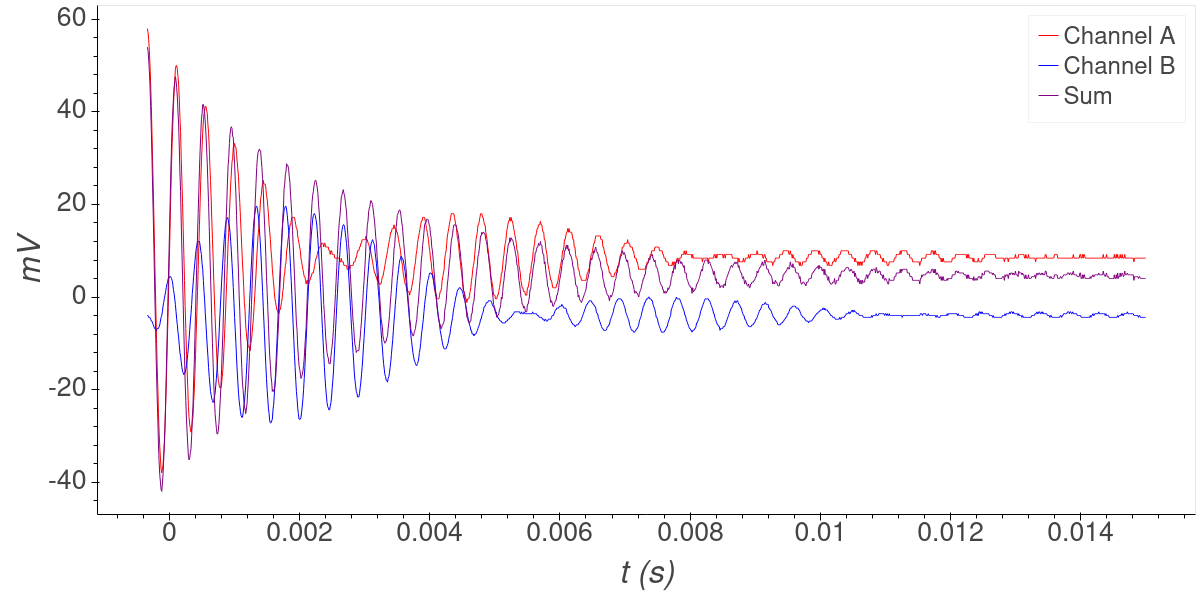
\includegraphics[width=0.48\textwidth]{../Images/l6_coupled_same_graph.png}
\caption{\label{waves} Two coupled LRC circuits, operating at a 90 degree
phase difference, and their sum.}
\end{figure}

We can see that the sum of the two channels produces a behavior very similar
to the uncoupled or individual LRC circuits, but each coupled circuit, when 
measured individually, expresses a ``beat" pattern.

\subsubsection{Discussion}

It is worth it to attempt to explain the behavior of the circuit before
moving on. It seems clear
that each time the A-capacitor discharges, most of the energy goes into
the A-inductor and bounces back in the typical oscillating fashion
seen above, but some of that energy goes into the B-circuit, producing a
pattern of oscillation there. With each oscillation, more energy is moved
into the B-circuit, but not as much energy is taken out of the B-circuit
by its own oscillations, so the energy in the B-circuit steadily grows. 
At a certain point, the energy leaving the A-circuit is less than the energy
leaving the B-circuit, and the pattern reverses, with the B-circuit
losing energy to the A-circuit until the A-circuit reaches another maxima. \\

However, because the energy lost by a given circuit is more or less the same
as the energy gained by the other one, the overall pattern of the sum of
energy in the circuit is the same as a single oscillator. Therefore it is
simply a translation of energy between two locations that produces this
``beat". \\

\subsection{Mechanical Analog}

This behavior is still a little inscrutable, and therefore it is
helpful to observe a mechanical analog which is more intuitively understood. 
This analog is a spring-mass system that is allowed to move in two dimensions, 
both up and down as well as side-to-side. A diagram describing this setup
can be found in fig. \ref{elastic pendulum}.

\begin{figure}[h]
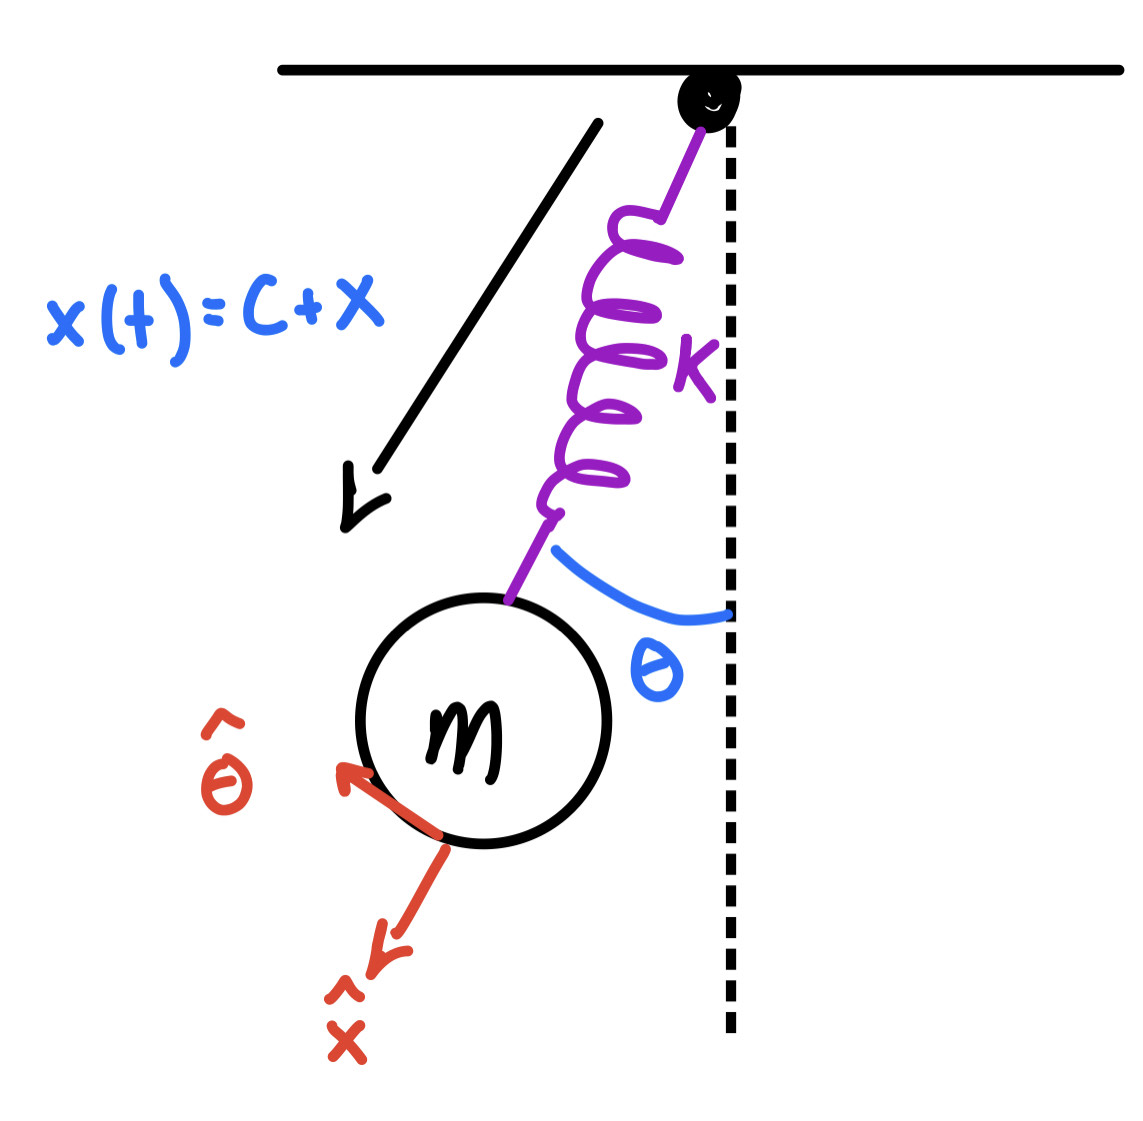
\includegraphics[width=0.48\textwidth]{../Images/l6_ElasticPendulum.jpg}
\caption{\label{elastic pendulum} Diagram of elastic pendulum coupled
mechanical oscillator.}
\end{figure}

This system was setup in the lab, and a demonstration was made. The motion
was initiated by simply adding tension to the string in the downward direction
and releasing. What was observed was a component of the motion, very small at
first, that was an angular, pendulum motion rather than a spring motion,
which grew slowly. At one point, this pendulum motion was the only motion 
observed, and the system by all means appeared to be a pendulum, for
about one period. However, at the end of this period, some small spring
motion was seen, which grew until the spring motion was the only motion
observed and there was no angular momentum, as in the initial condition.
This behavior then repeated several times. \\

This behavior is exactly like what was observed in the coupled LRC circuits,
but the distinction between the two forms of energy was more profound.
Instead of two waves that look similar, which are both described by the same
equations and the same parameters, the mechanical demonstration clearly
distinguished the exchange between the two forms of motion, angular and spring.
We can more clearly understand why energy is exchanged between these two
forms by thinking through it one step at a time, and we can draw parallels
to the coupled LRC system.\\

First, the spring is drawn back and released, close to directly below the
spring's mounting point. However, the mass is bound to be slightly off
center in some direction. There is very little pendulum motion in that
direction, but the accelerating spring gives a hard yank towards the
mounting point. This yank is harder than regular string tension would be,
if this was a regular pendulum, and the mass is kicked further out on
the other side of the mounting point. The same thing happens for some time,
until the spring is no longer providing a `yank' to the mass because it
is moving entirely in the pendulum mode with no motion toward or away from
the spring mounting point. However, this simple harmonic motion can't be
maintained because a spring does not provide the true tension force that
is needed to produce continuous motion, and will stretch rather than provide
a rigid restoring force. This stretching removes energy from the pendulum
system, which will no longer sweep as far out. That pattern continues until
the energy from the pendulum has been brought to zero, and we observe
a spring motion only. \\


\subsection{Fitting the ``Beat"}

In this section, numerical analysis is conducted on the digitized waveforms
in order to calculate the coupling capacitance. First, analysis is
simplified by fitting the inverse exponential to the sum of the two waves,
and then dividing each wave by the exponential to remove the effect of
the decay. This can be see in fig. \ref{nodecay}.

\begin{figure}[h]
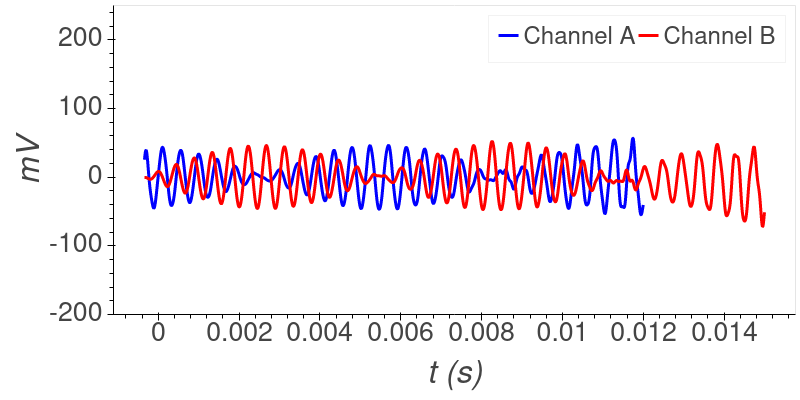
\includegraphics[width=0.48\textwidth]{../Images/l6_channels_sans_decay.png}
\caption{\label{nodecay} The resulting A and B channel waves after removing
the effect of the decay. A cutoff was chosen subjectively based on where the
noise was greater than the signal. }
\end{figure}

By using two approaches to curve fitting the beats, the beat frequency and
uncertainty were calculated. The first method involved taking the absolute
value of the signal, and then extracting every peak. A simpler Hilbert
transform approach was considered but the packet was not well defined enough
for this purpose. These peaks were then fit to a cosine wave, providing a
beat frequency for each wave. 

\begin{figure}[h]
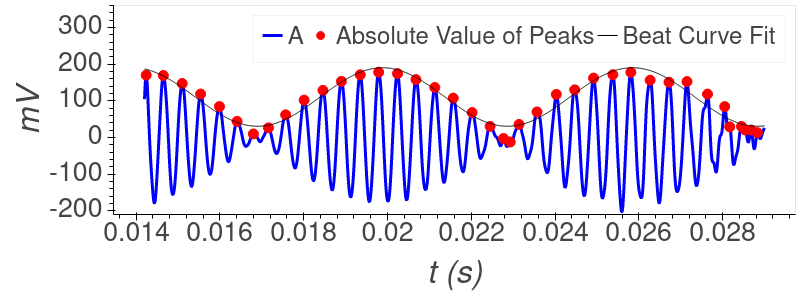
\includegraphics[width=0.48\textwidth]{../Images/l6_channel_A_peaks_fit.png}
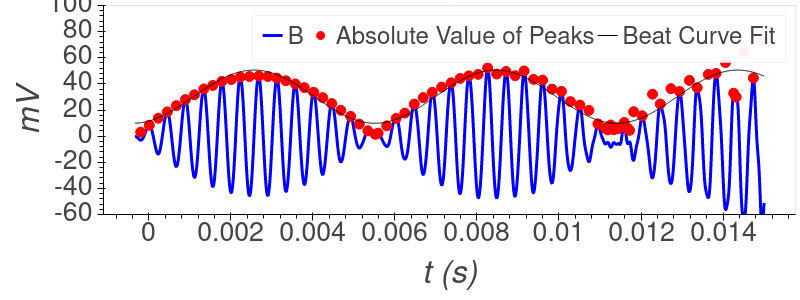
\includegraphics[width=0.48\textwidth]{../Images/l6_channel_B_peaks_fit.png}
\caption{\label{peaks_fits} Illustration of the peak fitting method of
curve fitting the beats for both A and B channel waves, with Channel A shown
above, and Channel B shown below.}
\end{figure}

The beat frequency for channel A was calculated at 168.34 Hz, and
the beat frequency for channel B was calculated at 171.77 Hz. \\

The second method for finding this beat frequency utilizes Fourier analysis.
The beat frequency is simply the difference between two dominant frequencies
at work in the signal, and these two frequencies will be obvious in the 
frequency domain, even if they are very difficult to compute in the time 
domain. The FFT of each wave was computed, with significant zero padding for
greater resolution and the hamming window to mitigate spectral leakage,
and the peak frequency from the two peaks was found.
The beat frequency is simply defined as the difference between the two peak
frequencies. The FFT analysis can be seen in fig. \ref{peaks}.

\begin{figure}[h]
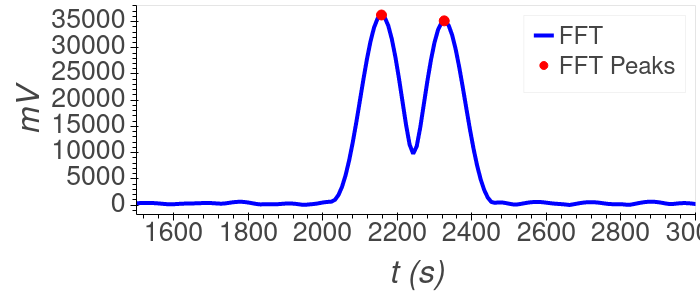
\includegraphics[width=0.48\textwidth]{../Images/l6_channel_A_fft.png}
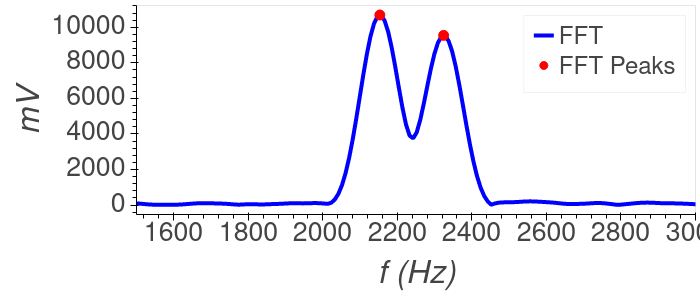
\includegraphics[width=0.48\textwidth]{../Images/l6_channel_B_fft.png}
\caption{\label{peaks} Illustration of the FFT method of curve fitting 
the beats for both A (above) and B (below) channel waves.}
\end{figure}

The peaks for channel A were located at 2153.06 and 2323.01 Hz, corresponding
to a beat frequency of 168 Hz. 
The peaks for channel B were located at 2153.01 and 2324.20 Hz, corresponding
to a beat frequency of 171 Hz. \\

These beat frequency measurements for each wave were then averaged
to produce a final calculated value, with the uncertainty taken as
the standard deviation across each of the two measurements. These
final values were 170 $\pm$ 1 Hz for channel A and 170.9 $\pm$ 0.9
for channel B. 

\subsection{Conclusion}

A derivation in appendix D details the differential equations describing 
the coupled LRC circuit without damping, assuming that the electrical
components used are identical.
The solution to the differential equations are shown below as

\begin{equation} 
q_+(t) = q_{+_0}sin(\omega_{+}t)
\label{qplus}
\end{equation}

\begin{equation} 
q_-(t) = q_{-_0}sin(\omega_{-}t)
\label{qplus}
\end{equation}

where q$_+$ = q$_1$ + q$_2$, q$_-$ = q$_1$ - q$_2$. q$_1$ and q$_2$ are 
the charges on the non-coupling capacitors in the coupled LRC circuits, and 
$\omega_-$ and $\omega_+$ are the frequencies of the oscillations of these
capacitor charges. From the derivation in Appendix D, the frequencies 
$\omega_-$ and $\omega_+$ are given by 

\begin{equation} 
\omega_+ = \frac{1}{2\pi\sqrt{LC}}
\label{omegaplus}
\end{equation}

\begin{equation} 
\omega_- = \frac{1}{2\pi\sqrt{L(C+C_{coup}}}
\label{omegaminus}
\end{equation}

where L is the inductance of the two inductors, C is the capacitance of the
two identical capacitors and C$_{coup}$ is the coupling capacitance.  \\

This system has two normal modes, as described earlier. When q$_1$ = q$_2$
at t = 0, $q_{-0}=0$ the two LRC circuits operate in phase with each other.
When q$_1$ = -q$_2$ at t = 0, $q_{+0} = 0$ the LRC circuits oscillate 
completely out of phase.\\

In the case of this experiment, q$_1$ = q$_0$ and q$_2$ = 0 at t = 0, because
A-capacitor has been fully charged by the square wave impulse, and B-capacitor
has been completely bypassed. For a coupled LRC circuit with these initial 
conditions the system behaves as a combination of the two normal modes.

\begin{equation} 
q = q_0(sin(\omega_{+}t)+sin(\omega_{-}t))
\label{Qeqn}
\end{equation}

For weak coupling, (C$_{coup}$  $<$ C), $\omega_{+}$ $\approx$ $\omega_{-}$,
and the normal modes are close in frequency. This gives rise to an apparent
``beat" in the charges on the two capacitors. By rewriting \ref{Qeqn} using
a trigonometric identity, this beat phenomena can more clearly be understood.

\begin{equation} 
q = 2q_0sin[(\frac{\omega_{+}+\omega_{-}}{2})t]cos[(\frac{\omega_{+}-\omega_{-}}{2})t]
\label{Qeqn2}
\end{equation}

Equation \ref{Qeqn2} is a characteristic equation describing beats,
or packets of waves. From Equation \ref{Qeqn2} the wave amplitude is 
determined by the sine term whereas the beat behavior is determined
by the cosine term. Thus for the initial conditions q$_1$ = q$_0$ and
q$_2$ = 0 at t = 0, with weak coupling, beats will be observed with a
frequency of $\omega_{+}$ $-$ $\omega_{-}$. These frequencies can
be substituted to produce the beat frequency as a function of
L, C, and $C_{coup}$.

\begin{equation} 
f_{beat} = \frac{1}{2\pi\sqrt{LC}}-\frac{1}{2\pi\sqrt{L(C+2C_{coup})}}
\label{fbeat}
\end{equation}

This equation can be rewritten to solve for the coupling capacitance.

\begin{equation} 
C_{coup} = \frac{1}{2}[\frac{1}{L(\frac{1}{\sqrt{LC}}-2\pi f_{beat})^2}-C]
\label{ccoup}
\end{equation}

Since the indicators and capacitors are identical within 
uncertainty, average values of L = 0.1 $\pm$ 0.003 H and C = 4.7 $\pm$ 0.1
nF were used. From these values, along with a beat frequency
f$_{beat}$ = 170 $\pm$1 Hz, the coupling capacitance C$_{coup}$ was 
calculated from Equation \ref{ccoup} to be 3.9 $\pm$0.1 nF.\\

This calculated value agrees with the assertion that the system had 
weak coupling, C$_{coup}$  $<$ C,and is very similar to the measured 
value of 4.1 $\pm$0.1 nF. \\

On a final note, the decision to analyze the falling edge of the pulse
generator should be commented on. The difference in behavior between
the rising edge and falling edge can be simply described as the falling
edge has more oscillations. The reason for this is found in the equation
for a single LRC circuit, shown below.

\begin{equation} 
	L \frac{d^2q}{dt^2} + R\frac{dq}{dt} + \frac{1}{C} q=0
\label{ccoup}
\end{equation}
With a non-zero voltage, the current will be much greater, meaning the
resistance will dissipate proportionally more energy, resulting in
more damping and fewer oscillations.



\section{Summary}

In this lab, the behavior of single, uncoupled, and coupled LRC circuits
were evaluated with simple relationships between L, R, C, and voltage
as well as complex differential equations. The latter were simplified
based on the unique initial conditions of this experiment. This behavior
was further linked to a mechanical analogue, a harmonic spring system. \\

In the first phase of the lab, basic quantities describing the circuit
and electrical components were measured directly, and calculated using
curve fits which relate to solutions to the differential equations describing
LRC oscillations. These values are summarized below, in Table I. In these
calculations, it was observed that the precision of the DMM was responsible
for virtually all of the uncertainty in our measurements. \\

In the second phase of the lab, the two circuits were coupled via a
capacitor, which adds immense complexity to the differential equations
describing the flow of charge. It was, however, possible to relate the
beat frequency, or the difference in the fundamental frequency of the
two circuits A and B, to the capacitance of the coupling capacitor $C_coup$
using some assumptions related to the initial conditions of the circuits
and building on more accessible solutions to these governing equations
known as `normal' operating modes. \\

It was possible to find this beat frequency by doing analysis on the
signals from each channel in the time and frequency domain. By
dividing the effect of damping out of the signals, then fitting
the amplitude of the peaks, the changing amplitude of each wave was matched
with a beat frequency. Separately, by simply finding the fundamental
frequency of the two added waves which produce the beat using the FFT,
the beat frequency could be found more directly. Both methods were 
considered to produce the final measure of beat frequency, 170 $\pm$ 1 Hz 
for each channel A and B. This agreement makes sense considering the
beat is caused by the difference in each circuits own operating frequency
and the other's. \\

Using these measurements of beat frequency, the final value for $C_{coup}$
was calculated at 4.1 $\pm$ 0.1 nF, which is in close agreement with the
measured value of 3.9 $\pm$ 0.1 nF. Given the amount of calculations needed,
this value is satisfyingly close at 1 sigma. Some of this error may
be due to discrepancies in the A and B circuits. If they are not perfectly
identical, then the assumptions behind our equations are not accurate and
the effective capacitance and resistance of the circuit, for example,
will be different than expected.


\newpage
\begin{widetext}
\begin{center}
\begin{table}[h]
\renewcommand{\arraystretch}{1.35}
\setlength{\tabcolsep}{10pt}
\caption{\label{DONE BITCH}Measured and calculated values from analysis of the two inductors in the individual LRC circuit.}
\begin{tabular}{|c|c|c|}
%\hline
\toprule
Inductor Label & 'A' & 'B'\\
\colrule
Full Decay Natural Frequency, $\omega_0$ & 14587.05  $\pm$ 0.03 rad/s & 14578.44 $\pm$ 0.03 rad/s \\
\colrule
Damping Constant, $\gamma$ & 649.9 $\pm$ 0.1  $s^{-1}$ & 651.3 $\pm$ 0.1  $s^{-1}$  \\
\colrule
Single Period Inductance, L & 0.099 $\pm$ 0.009 H &  0.101 $\pm$ 0.009 H\\
\colrule
Full Decay Inductance, L & 0.100 $\pm$ 0.003 H & 0.100 $\pm$ 0.003 H \\
\colrule
Calculated Resistance, R & 65 $\pm$ 2 $\Omega$ & 65 $\pm$ 2 $\Omega$ \\
\colrule
Measured Resistance, R & 17.4 $\pm$ 0.5 $\Omega$ & 17.2 $\pm$ 0.5 $\Omega$ \\
\colrule
Time Constant, $\tau$ & 3077.3 $\pm$ 0.6 $\mu$s & 3070.9 $\pm$ 0.6 $\mu$s\\
\colrule
Quality Factor, Q & 22.4 $\pm$ 0.3 & 22.4 $\pm$ 0.3\\
%\hline
\botrule
\end{tabular}
\end{table}

\begin{table}[h]
\renewcommand{\arraystretch}{1.35}
\setlength{\tabcolsep}{10pt}
\caption{\label{DONE BITCH 2}Measured calculated values from the analysis of the coupled LRC circuits.}
\begin{tabular}{|c|c|c|c|}
%\hline
\toprule
Property & Calculated Value & Measured Value & Deviation \\
\colrule
LRC Capacitence & Standard / 'A': 47.1 $\pm$ 1 nF & Variable / 'B': 47.1 $\pm$ 1 nF & 0$\sigma$\\
\colrule
Beat Frequency & Circuit 'A' Beats: 170 $\pm$ 1 Hz & Circuit 'B' Beats: 170.9 $\pm$ .9 Hz & - \\
\colrule
Coupling Capacitance &  4.1 $\pm$0.1 nF & 3.9 $\pm$0.1 nF & 1$\sigma$\\


%\hline
\botrule
\end{tabular}
\end{table}
\end{center}
\end{widetext}


\newpage
\begin{thebibliography}{9}
%

\bibitem{Feynman} \\
S. Strogatz, \textit{“Infinite Powers: How Calculus Reveals the Secrets of the Universe”}, (Houghton Mifflin Harcourt, New York, 2019).
%
\\\\\\\\
\bibitem{Ficks} 
Oregon Graduate Institute, Diffusion Theory: Fick's Laws: \\
\href{https://omlc.org/classroom/ece532/class5/ficks1.html}{https://omlc.org/classroom/ece532/class5/ficks1.html}

\bibitem{Heat} 
Stanford, Heat Equation: \\
\href{https://web.stanford.edu/class/math220b/handouts/heateqn.pdf}{https://web.stanford.edu/class/math220b/handouts/heateqn.pdf}


\bibitem{NS} 
NASA, Navier-Stokes Equations: \\
\href{https://www.grc.nasa.gov/www/k-12/airplane/nseqs.html}{https://www.grc.nasa.gov/www/k-12/airplane/nseqs.html}
%
\bibitem{Lenz} 
Wikipedia, Lenz's Law: \\
\href{https://en.wikipedia.org/wiki/Lenz27s_law}{https://en.wikipedia.org/wiki/Lenz27s_law}


\end{thebibliography}




\end{document}
%
% ****** End of file apstemplate.tex ******

